\documentclass[12pt]{article}
\textwidth=17cm \oddsidemargin=-0.9cm \evensidemargin=-0.9cm
\textheight=23.7cm \topmargin=-1.7cm

\usepackage{amssymb, amsmath, amsfonts}
\usepackage{moreverb}
\usepackage{graphicx}
\usepackage{enumerate}
\usepackage{graphics}
\usepackage{color}
\usepackage{array}
\usepackage{float}
\usepackage{smartdiagram}
\usepackage{hyperref}
\usepackage{textcomp}
\usepackage{alltt}
\usepackage{physics}
\usepackage{mathtools}
\usepackage{tikz}
\usetikzlibrary{positioning,arrows,matrix,shapes,decorations.text}
\usepackage{pgfplots}
\pgfplotsset{compat=1.10}
\usepackage{bigints}
\allowdisplaybreaks

\newcommand{\suchthat}{\, \mid \,}
\renewcommand{\theenumi}{\alph{enumi}}
\newcommand\Wider[2][3em]{%
\makebox[\linewidth][c]{%
  \begin{minipage}{\dimexpr\textwidth+#1\relax}
  \raggedright#2
  \end{minipage}%
  }%
}

\setcounter{section}{-1}

\title{\bf HW \#1}
\author{\bf Writer: Sam Fleischer \\ \bf Carter Johnson \\ \bf Xiaoyun Niu}
\date{\bf October 5, 2015}

\begin{document}
{\bf MATH 207A \hfill Applied Mathematics \ \ \ \ \hfill Fall 2015} 

{\let\newpage\relax\maketitle}

\section*{Problem 1}
{\it Consider the following chemical reaction, where one chemical ($A$) turns into a different chemical ($B$) and vice versa.  Suppose that the total amount of chemical is constant, that is $A(t) + B(t) = C$, where $C$ is a positice constant.  This reaction can be represented schematically in the following way:}
\begin{center}
	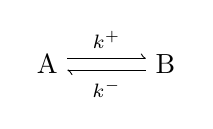
\begin{tikzpicture}
	    \node (A) at (0,0) {A};
	    \node (B) at (1.5,0) {B};
		\begin{scope}[every node/.style={font= \scriptsize}]
			\draw[transform canvas={yshift=0.5ex},-left to] (A) -- node[above]{$k^+$}  (B);
			\draw[transform canvas={yshift=-0.5ex},left to-] (A) -- node[below] {$k^-$} (B); 
		\end{scope}
	\end{tikzpicture} 
\end{center}
{\it where the two positive constants $K^+$ and $k^-$ are called rate constants.}

{\it The following differential equation describes how $A$ changes with time}
\begin{equation}
	\label{change_chem_A}
	\frac{\dd A}{\dd t} = -k^+ A + k^- B
\end{equation}
{\it Recall that, in addition to this differential equation, we have the conservation constraint $A(t) + B(t) = C$.}

\subsection*{ a)}
{\it Solve for $A(t)$, given $A(0) = A_0$, with $A_0$ being a positive constant such that $A_0 < C$.} \\

Eq.~(\ref{change_chem_A}) can be simplified by using the conservation constraint as
\begin{align*}
	\frac{\dd A}{\dd t} &= -k^+ A + k^- \qty(C - A) \\
	&= -\qty(k^+ + k^-)A + k^-C
\end{align*}
Let $u(t) = -\qty(k^+ + k^-)A(t) + k^-C$.  Then $\dot{u} = -\qty(k^+ + k^-)\dot{A}$.  Thus,
\begin{equation}
	\label{change_chem_u}
	\dot{u} = -(k^+ + k^-)u
\end{equation}
The solution to Eq.~(\ref{change_chem_u}) is exponential, i.e.
\begin{align*}
	u(t) &= Z\exp\qty(-(k^+ + k^-)t)\ \ \ \ \text{for some arbitrary constant $Z$} \\
	\implies A(t) &= Z\exp\qty(-(k^+ + k^-)t) + \frac{k^-C}{k^+ + k^-}
\end{align*}
The initial condition $A(0) = A_0$ implies
\begin{align*}
	Z = A_0 - \frac{k^-C}{k^+ + k^-}
\end{align*}
and so
\begin{equation}
	\label{chem_solution}
	A(t) = \qty(A_0 - \frac{k^-C}{k^+ + k^-})\exp\qty(-(k^+ + k^-)t) + \frac{k^-C}{k^+ + k^-}
\end{equation}

\subsection*{ b)}
{\it Use Matlab to check your answer for a few choices of $A_0$, $C$, $k^+$, and $k^-$ (I have provided code that will assist you).}

\begin{center}
	\includegraphics[width=400px]{figures/1_b_1.png}
	\includegraphics[width=400px]{figures/1_b_2.png}
\end{center}

\section*{Problem 2}
{\it The position of a moving object in 1-D ($x(t)$) on a damped linear spring obeys the following differential equation}
\begin{equation}
	\label{change_position}
	m\ddot{x} = -b\dot{x} - kx
\end{equation}
{\it where $m$, $b$, and $k$ are positive constants representing the mass of the object, the damping coefficient and the stiffness of the spring, respectively.}

\subsection*{ a)}
{\it Solve for $x(t)$, given $x(0) = x_0$ and $\dot{x}(0) = v_0$.} \\

Since Eq.~(\ref{change_position}) is a linear ODE, we can solve for the roots the characteristic polynomial, which is
\begin{align*}
	P(\lambda) &= m\lambda^2 + b\lambda + k = 0 \\[.2cm]
	\implies \lambda_{1,2} &= \frac{-b \pm \sqrt{b^2 - 4mk}}{2m}
\end{align*}
and thus the solution to Eq.~(\ref{change_position}) is
\begin{align*}
	\label{general_soluntion}
	x(t) =  \left\{\begin{array}{ll}
		C_1\exp\qty(\lambda_1 t) + C_2\exp\qty(\lambda_2 t) & \text{if $\lambda_1 \neq \lambda_2$ and $\lambda_1,\lambda_2 \in \mathbb{R}$} \\[.1cm]
		C_1\exp\qty(\lambda t) + C_2 t\exp\qty(\lambda t) & \text{if $\lambda_1 = \lambda_2 = \lambda \in \mathbb{R}$} \\[.1cm]
		C_1\exp\qty(\alpha t)\sin\qty(\beta t) + C_2\exp\qty(\alpha t)\cos\qty(\beta t) & \text{if $\lambda_{1,2} = \alpha \pm \beta i \in \mathbb{C}$}
	\end{array}\right.
\end{align*}
The conditions simplify based on the formulation of $\lambda_{1,2}$ to
\begin{equation}
	\label{general_soluntion}
	x(t) =  \left\{\begin{array}{ll}
		C_1\exp\qty(\lambda_1 t) + C_2\exp\qty(\lambda_2 t) & \text{if $b^2 - 4mk > 0$} \\[.1cm]
		C_1\exp\qty(\lambda t) + C_2 t\exp\qty(\lambda t) & \text{if $b^2 - 4mk = 0$} \\[.1cm]
		C_1\exp\qty(\alpha t)\sin\qty(\beta t) + C_2\exp\qty(\alpha t)\cos\qty(\beta t) & \text{if $b^2 - 4mk < 0$}
	\end{array}\right.
\end{equation}

\subsubsection*{Case 1: $b^2 - 4mk > 0$}
\begin{align*}
	x(t) &= C_1\exp\qty(\lambda_1 t) + C_2\exp\qty(\lambda_2 t) \\
	\dot{x}(t) &= C_1\lambda_1\exp\qty(\lambda_1 t) + C_2\lambda_2\exp\qty(\lambda_2 t)
\end{align*}
Since $x(0) = x_0$ and $\dot{x}(0) = v_0$,
\begin{align*}
	&x_0 = C_1 + C_2\ \ \text{and}\ \ v_0 = C_1\lambda_1 + C_2\lambda_2 \\[.1cm]
	\implies &C_1 = \frac{x_0\lambda_2 - v_0}{\lambda_2 - \lambda_1}\ \ \text{and}\ \ C_2 = \frac{x_0\lambda_1 - v_0}{\lambda_1 - \lambda_2} \\[.1cm]
	\implies &\boxed{x(t) = \frac{x_0\lambda_2 - v_0}{\lambda_2 - \lambda_1}\exp\qty(\lambda_1 t) + \frac{x_0\lambda_1 - v_0}{\lambda_1 - \lambda_2}\exp\qty(\lambda_2 t)}
\end{align*}

\subsubsection*{Case 2: $b^2 - 4mk = 0$}
\begin{align*}
	x(t) &= C_1\exp\qty(\lambda t) + C_2t\exp\qty(\lambda t) \\
	\dot{x}(t) &= C_1\lambda\exp\qty(\lambda t) + C_2\lambda t\exp\qty(\lambda t) + C_2\exp\qty(\lambda t)
\end{align*}
Since $x(0) = x_0$ and $\dot{x}(0) = v_0$,
\begin{align*}
	&x_0 = C_1\ \ \text{and}\ \ v_0 = C_1\lambda + C_2 \\[.1cm]
	\implies &C_1 = x_0\ \ \text{and}\ \ C_2 = v_0 - x_0\lambda \\[.1cm]
	\implies &\boxed{x(t) = x_0\exp\qty(\lambda t) + (v_0 - x_0\lambda)t\exp\qty(\lambda t)}
\end{align*}

\subsubsection*{Case 3: $b^2 - 4mk < 0$}
\begin{align*}
	x(t) &= C_1\exp\qty(\alpha t)\sin\qty(\beta t) + C_2\exp\qty(\alpha t)\cos\qty(\beta t) \\
	\dot{x}(t) &= C_1\qty(a\exp\qty(\alpha t)\sin\qty(\beta t) + b\exp\qty(\alpha t)\cos\qty(\beta t)) + C_2\qty(a\exp\qty(\alpha t)\cos\qty(\beta t) - b\exp\qty(\alpha t)\sin\qty(\beta t))
\end{align*}
Since $x(0) = x_0$ and $\dot{x}(0) = v_0$,
\begin{align*}
	&x_0 = C_2\ \ \text{and}\ \ v_0 = C_1 \beta + C_2 \alpha \\[.1cm]
	\implies &C_1 = \frac{v_0 - x_0 \alpha}{\beta}\ \ \text{and}\ \ C_2 = x_0 \\[.1cm]
	\implies &\boxed{x(t) = \frac{v_0 - x_0 \alpha}{\beta}\exp\qty(\alpha t)\sin\qty(\beta t) + x_0\exp\qty(\alpha t)\cos\qty(\beta t)}
\end{align*}

\subsection*{ b)}
{\it Use Matlab to check your answer for a few choices of $x_0$, $v_0$, $b$, $m$, and $k$ (I have provided code that will assist you).}

\begin{center}
	\includegraphics[width=400px]{figures/2_b_decay_1.png}
	\includegraphics[width=400px]{figures/2_b_decay_2.png}
	\includegraphics[width=400px]{figures/2_b_oscillation_1.png}
	\includegraphics[width=400px]{figures/2_b_oscillation_2.png}
\end{center}

\subsection*{ c)}
{\it Assuming that both $x_0$ and $v_0$ are not zero, what inequality must $m$, $b$, and $k$ satisfy in order to given an oscillatory solution (i.e. a solution $x(t)$ that contains sine/cosine terms)?} \\

From part a), the solution is only oscillatory if $b^2 - 4mk < 0$.  The period of the oscillations depend on $\text{Im}[\lambda] = \beta$.  The magnitude of the oscillations depend on $\text{Re}[\lambda] = \alpha$.  If $\alpha > 0$ then the magnitude of the oscillations will grow exponentially, if $\alpha < 0$ then the magnitude of the oscillations will decay exponentially, and if $\alpha = 0$, then the magnitude of the oscillations will stay constant.  However, we know $\alpha$ = $\frac{-b}{2m}$, where $b$ and $m$ are positive constants, and so $\alpha < 0$, resulting in decaying oscillations.

\section*{Problem 3}
{\it The following equation describes the velocity $v(t)$ of a relatively large object falling through and inviscid medium (e.g.~a baseball falling through the air)}
\begin{equation}
	\label{change_bead}
	m\dot{v} = -cv|v| + mg
\end{equation}
{\it where $m$, $c$, and $g$ are positive constants representing the mass of the object, the drag of the fluid and the pull of gravity, respectively.}

\subsection*{ a)}
{\it Draw a plot of $\dot{v}$ vs.~$v$.  Label any fixed point(s) and indicate the stability of each.  On the horizontal axis ($v$), indicate the flow direction.}

\begin{center}
	\includegraphics[width=400px]{figures/3_a.jpg}
\end{center}

\subsection*{ b)}
{\it Without solving the equation, sketch $v(t)$ as a function of $t$ for several initial conditions.}

\begin{center}
	\includegraphics[width=400px]{figures/3_b.jpg}
\end{center}

\subsection*{ c)}
{\it Solve the equation for $v(t)$ given $v(0) = 0$.  (It will simplify your life considerably to assume that $v \geq 0$ to get rid of the absolute value sign.  Once you have a solution, you can determine whether this is a reasonable assumption.)} \\

First, assume $v \geq 0$, and thus $m\dot{v} = -cv^2 + mg$.  Eq.~(\ref{change_bead}) is a separable equation, i.e.
\begin{align*}
	m\int \frac{\dd v}{mg - cv^2} = \int \dd t
\end{align*}
The left hand side integral requires partial fractions:
\begin{align*}
	\frac{1}{mg - cv^2} &= \frac{A}{\sqrt{mg} - \sqrt{c}v} + \frac{B}{\sqrt{mg} + \sqrt{c}v} \\[.1cm]
	\implies 1 &= \qty(A + B)\sqrt{mg} + \qty(B - A)\sqrt{c}v \\
	\implies A &= B = \frac{1}{2\sqrt{mg}}
\end{align*}
and thus,
\begin{align*}
	\frac{\sqrt{m}}{2\sqrt{g}}\qty(\int \frac{\dd v}{\sqrt{mg} - \sqrt{c}v} + \int \frac{\dd v}{\sqrt{mg} - \sqrt{c}v}) = \int \dd t
\end{align*}
Using $u$-substitution ($u = \sqrt{mg} \pm \sqrt{c}v$),
\begin{align*}
	\int \frac{\dd v}{\sqrt{mg} - \sqrt{c}v} &= -\frac{1}{\sqrt{c}}\int\frac{\dd u}{u} = -\frac{\ln\qty(\sqrt{mg} - \sqrt{c}v)}{\sqrt{c}}\ \ \text{and} \\[.1cm]
	\int \frac{\dd v}{\sqrt{mg} + \sqrt{c}v} &= \frac{1}{\sqrt{c}}\int\frac{\dd u}{u} = \frac{\ln\qty(\sqrt{mg} + \sqrt{c}v)}{\sqrt{c}}
\end{align*}
Thus,
\begin{align*}
	\frac{\sqrt{m}}{2\sqrt{cg}}\ln\qty(\frac{\sqrt{mg} + \sqrt{c}v}{\sqrt{mg} - \sqrt{c}v}) = t + C\ \ \ \text{for some arbitrary constant $C$}
\end{align*}
The initial condition $v(0) = 0$ implies $C = 0$.  Then the above can be solved for $v$:
\begin{equation}
	\label{bead_solution}
	v(t) = \frac{\sqrt{mg}\qty(\exp\qty(\frac{2\sqrt{cg}}{\sqrt{m}}t) - 1)}{\sqrt{c}\qty(\exp\qty(\frac{2\sqrt{cg}}{\sqrt{m}}t) + 1)}
\end{equation}
Since $\frac{2\sqrt{cg}}{\sqrt{m}} > 0$ and $t \geq 0$, then $\exp\qty(\frac{2\sqrt{cg}}{\sqrt{m}}t) \geq 1$, which implies $v(t) \geq 0$ for all $t > 0$.  Thus our assumption ($v \geq 0$) is still reasonable.

\subsection*{ d)}
{\it Use Matlab to check your solution.  I have not provided code, but you should be able to modify the code for Problem 1.}

\begin{center}
	\includegraphics[width=400px]{figures/3_d_1.png}
	\includegraphics[width=400px]{figures/3_d_2.png}
\end{center}

\section*{Problem 4}
{\it The DNA in your body codes for specific proteins.  Proteins affect how cells in your body behave - even whether they live or die.  In some cells, you might want a high concentration of a particular protein; in other cells, you might want only a small concentration of that protein.}\\

\begin{figure}[h]
	\centering
	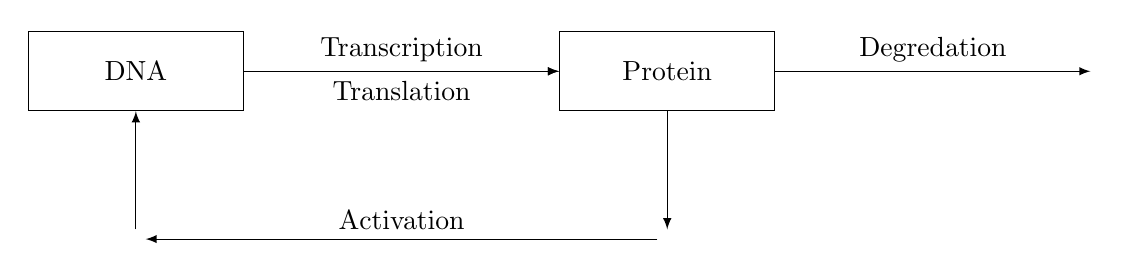
\begin{tikzpicture}[
	node distance=1.5cm and 4cm,
	ar/.style={->,>=latex},
	mynode/.style={
	  draw,
	  text width=2.5cm,
	  minimum height=1cm,
	  align=center
	  }
	% mypostaction/.style 2 args={
	%   decoration={
	%     text align={
	%       left indent=#1},
	%       text along path, 
	%       text={#2}
	%     },
	%   decorate
	% }
	]
		\node[mynode] (dna) {DNA};
		\node[mynode,right=of dna] (pro) {Protein};
		\node[right=of pro] (nowhere) {};
		\node[below=of pro] (below_pro) {};
		\node[below=of dna] (below_dna) {};


		\draw[ar] 
			(dna) -- node[above] {Transcription} (pro);
		\draw[ar] 
			(dna) -- node[below] {Translation} (pro);
		\draw[ar]
			(pro) -- node[above] {Degredation} (nowhere);
		\draw[ar]
			(pro) -- node[above] {} (below_pro);
		\draw[ar]
			(below_pro) -- node[above] {Activation} (below_dna);
		\draw[ar]
			(below_dna) -- node[above] {} (dna);
		% \draw[->]
		% 	(pro) to [out=-90,in=-90] (dna);
		% \path[postaction={mypostaction={3.4cm}{Activation}, /pgf/decoration/raise=1.5mm}]
		% 	(dna) to[out=-90,in=-90,looseness=1] (pro);
	\end{tikzpicture}
	\label{Figure_1}
	\caption{DNA/Protein Interface}
\end{figure}

{\it Cells in your body typically destroy proteins; they have only a finite lifetime.  Thus, the amount of a particular protein in one of your cells at a given time, $p(t)$, is determined by a balance between the rate of protein formation and destruction.  Sometimes, the amount of protein affects how fast protein is made.  Here we consider such a situation, as shown schematically in \emph{Figure 1} above.

Mathematically, the system can be expressed with the following equation:}
\begin{align*}
	\label{change_protein}
	\dot{p} = -kp + A\frac{p^2}{p^2 + B^2}
\end{align*}
{\it where $k$, $A$, and $B$ are positive constants that determine how quickly the protein is destroyed, how quickly the protein is formed, and how strongly the protein affects its formation, respectively.  For simplicity, assume that $k = B = 1$.}

\subsection*{ a)}
{\it Assuming that $k = B = 1$, draw a phase protrait for the case where $A = 6$ (i.e.~plot $\dot{p}$ vs.~$p$, indicate any fixed point(s) and indicate the stability of each.  On the horizontal axis ($p$) indicate the flow direction of phase points).} 

\begin{center}
	\includegraphics[width=400px]{figures/4_a.jpg}
\end{center}

\subsection*{ b)}
{\it Without solving the equation, sketch $p(t)$ as a function of $t$ for several initial conditions for $A = 6$.} 

\begin{center}
	\includegraphics[width=400px]{figures/4_b.jpg}
\end{center}

\subsection*{ c)}
{\it Assuming that $k = B = 1$, draw a phase protrait for the case where $A = 1$ (i.e.~plot $\dot{p}$ vs.~$p$, indicate any fixed point(s) and indicate the stability of each.  On the horizontal axis ($p$) indicate the flow direction of phase points).} 

\begin{center}
	\includegraphics[width=400px]{figures/4_c.jpg}
\end{center}

\subsection*{ d)}
{\it Without solving the equation, sketch $p(t)$ as a function of $t$ for several initial conditions for $A = 1$.} 

\begin{center}
	\includegraphics[width=400px]{figures/4_d.jpg}
\end{center}

\subsection*{ e)}
{\it Suppose you wanted to maintain a non-zero steady-state concentration of protein in one of your cells.  Would you choose $A = 1$ or $A = 6$?  What else would you have to do to ensure a non-zero steady state?} \\

Clearly, if $A = 1$, there is only one stable fixed point: the trivial fixed point $p_0 = 0$.  However, if $A = 6$ there are three fixed points: the trivial fixed point $p_0 = 0$, which is stable, an unstable non-zero fixed point $p_1 \approx 0.1716$, and a stable non-zero fixed point $p_2 \approx 5.8284$.  Thus, if we want to maintain a non-zero steady-state concentration of protein in one of our cells, we should choose $A = 6$.  We also need to ensure the initial condition $p(0) > p_1$.  This way, all solutions send the protein concentration to $p_2$.  If $p(0) = p_1$, a negative perturbation would send the protein concentration to $0$.  If $p(0) < p_1$, all solutions send the protein concentration to $0$.

\end{document}
